\subsection{Numerical Method Performance}
We evaluated the efficiency of each numerical approach by varying the step size, $h$ to achieve a comparable absolute error among all methods.

The step size $h$ or tolerances for adaptive methods are picked such that the maximum absolute error is within $10^{-2}$ of our reference equation.

With the initial conditions as described in Table ~\ref{tab:constants}, simulations were run with all 5 models across 24 months. 
All models indicate the extinction of species $x$ with population $y$ limited by its independent-species carrying capacity, $K_2$, as seen in Figure ~\ref{fig:methods}.
All methods but Euler's method converged to a maximum absolute error of $10^{-2}$, as Euler's very poor error convergence of $\mathcal{O}(h)$ would require computational power beyond what was available for this project.
Calculated maximum absolute errors and size of $h$ can be seen in Table ~\ref{tab:performance}.
Tolerances for both RKF45 and DP45 were set between $10^{-3}$ and $10^{-1}$, with step sizes between $10^{-2}$ and $10^{-1}$.

\begin{table}[htbp]
\centering
\caption{Numerical Method Performance}
\label{tab:performance}
\begin{tabular}{@{}lll@{}}
\toprule
\textbf{Numerical Method} & \textbf{Max Absolute Error} & \textbf{Step Size $h$} \\ 
\midrule
Euler & $6.77 \times 10^{0}$ & 1 minute \\
Improved Euler & $1.56 \times 10^{-2}$ & 15 minutes \\
RK4 & $6.819750 \times 10^{-2}$ & 2 days \\
RKF45 & $5.246770 \times 10^{-2}$ & 3.04 hours (average) \\
DP45 & $1.261326 \times 10^{-2}$ & 3.04 hours (average) \\
\bottomrule
\end{tabular}
\end{table}

\begin{figure}[!h]
    \centering
    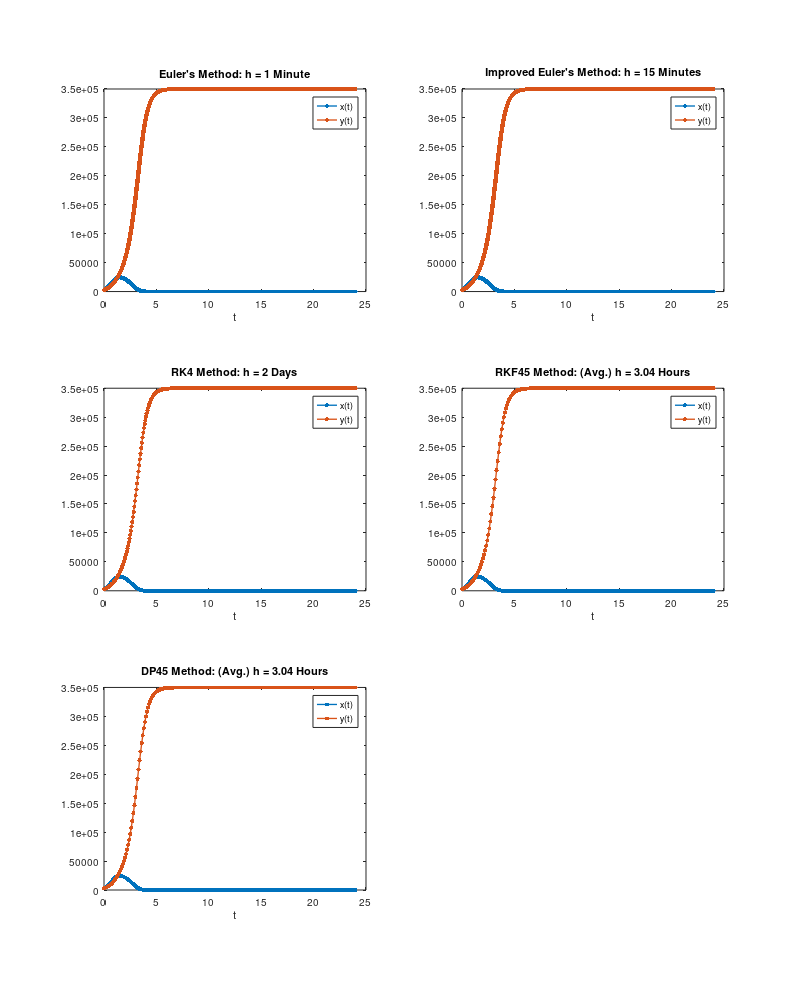
\includegraphics[width=1.0\textwidth, height=0.85\textheight, keepaspectratio]{Figures/methodscomparison.png}
    \caption{Results of all numerical methods with initial conditions from Table ~\ref{tab:constants} from $t = 0$ to $t= 24$ with specified step size $h$.}
    \label{fig:methods}
\end{figure}

From the results, we can determine that our most efficient method here is RK4, with $h = 2$ days. DP45 and RKF45 perform well with $h = 3.04$ hours. For $t<5$, $h$ is relatively large, but as $y$ approaches $k2$, $h$ shrinks dramatically, decreasing the average step size down.


\subsection{Competing Species}
Results of Figure ~\ref{fig:methods} also show that under the given conditions, we reach a stable solution in which $y$ reaches and sustains its independent-species carrying capacity, $K_2$. 
While $x$ initially rises due to its high birth rate, the carrying capacity of $K_1$ is much higher than $K_2$, and therefore its growth is immediately limited. 
The greater increase in $y$ also increases the weight of the term $c_2xy$ in Equation 2, further decreasing the density of the population $x$.

By modifying our initial constants from Table ~\ref{tab:constants}, we can change the surviving population from species $y$ to species $x$. 
One such way is to decrease the birthrate of $y$, $\beta_2$. 
By limiting $\beta_2$, drivers of $x$ outpace those of $y$, while $x \gg y$ reduces population $y$ to extinction.
The value for $\beta_2$ was varied according to binary search to determine the point of bifurcation in which either population wins out, and was determined to a precision of $10^{-15}$ to be:
$$\beta_2 = 1.003294587846742\dots$$
This is not an exact value, and cannot be expressed in terms of other constants, as it depends highly on initial populations and other scenario-specific consequences of the model.
When $\beta_2 < 1.00329\dots$ population $x$ becomes the surviving population, while $\beta_2 > 1.00329\dots$ results in a surviving population $y$.
When exactly equal, numerical methods predict that a metastable solution exists in which both species can coexist, but this is simply an artifact of binary precision.

Alternatively, it is possible for both species to coexist, just not by variation of $\beta_2$ alone. In fact, coexistence can be ensured if the following conditions are met by the initial parameters:
\begin{equation}
\label{eq:stability-conditions}
\begin{aligned}
    \beta_1 &> c_1 K_2 \\
    \beta_2 &> c_2 K_1
\end{aligned}
\end{equation}
This is derived from a 2018 paper \cite{Gavina2018}, with the following equations for their competing species: 

$$
    x' = \beta_1 x \left(1 - \frac{x + \alpha_{12} y}{K_1}\right)
$$

$$
    y' = \beta_2 y \left(1 - \frac{y + \alpha_{21} x}{K_2}\right)
$$

Noticeably, this is extremely similar to our competing species model with their respective $\beta$'s factored out: 

$$
    x' = \beta_1 x \left(1 - \frac{x}{K_1} - \frac{c_1}{\beta_1}y\right)
$$

$$
    y' = \beta_2 y \left(1 - \frac{y}{K_2} - \frac{c_2}{\beta_2}x\right)
$$

Our models then become exactly the same if their $\alpha_{12}$ is set equal to $\frac{c_1 K_1}{\beta_1}$, and if their  $\alpha_{21}$ is set equal to $\frac{c_2 K_2}{\beta_2}$. In their paper they have an inequality that guarantees coexistence: 

$$
    K_1 > \frac{K_2}{\alpha_{21}}
$$

$$
    K_2 > \frac{K_1}{\alpha_{12}}
$$

This inequality becomes the aforementioned inequality~\ref{eq:stability-conditions} applicable to our model when $ \alpha_{12}$ and $\alpha_{21}$ are correctly substituted. Then, coexistence is as simple as choosing values that satisfy our inequality derived from theirs. As is, condition 1 of the inequality is violated: 

$$
    \beta_1 > c_1 K_2 \quad\Rightarrow\quad 3.15 > (3\times10^{-5})(3.5\times10^5) = 10.5
$$

$$
    \beta_2 > c_2 K_1 \quad\Rightarrow\quad 2.1 > (3\times10^{-5})(3.5\times10^4) = 1.05
$$

Hence why coexistence could not be ensured by varying $\beta_2$ alone; the first inequality will always be false regardless of $\beta_2$. Arbitrarily, we chose $\beta_1=12$ to satisfy the first condition, which, as expected, led to coexistence shown in Figure ~\ref{fig:coexistence}.

\begin{figure}[!h]
    \centering
    % Adjust [width=0.8\textwidth] if you want it larger or smaller on the page
    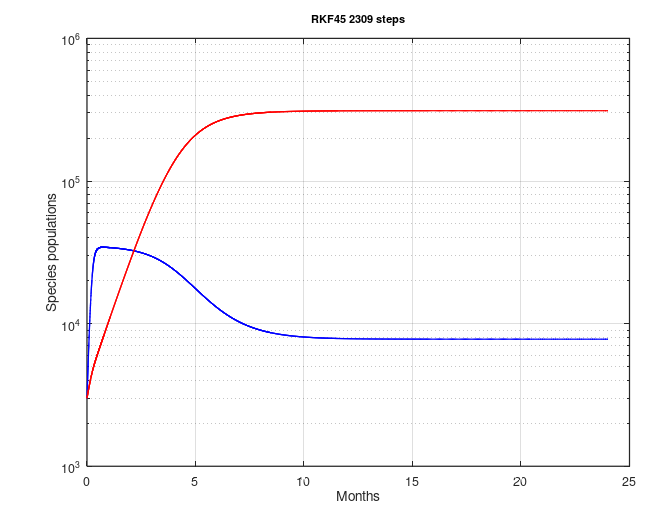
\includegraphics[width=1.0\textwidth, height=0.85\textheight, keepaspectratio]{Figures/coexistnopredator.png}
    \caption{Coexistence of prey populations meeting the inequalities of Equation ~\ref{eq:stability-conditions}.}
    \label{fig:coexistence}
\end{figure}


\subsection{Introducing a Predator}
Upon introducing a predator population, we reset our initial parameters defined in Table ~\ref{tab:constants}, and tested initial predator population densities $z_0=1... 20$, seen in Figure ~\ref{fig:predator}.

\begin{figure}[h]
    \centering
    % {10} is frame rate, {Figures/frame-} is the path + file prefix
    \animategraphics[loop, autoplay, width=0.8\textwidth]{10}{Figures/frame-}{0}{19}
    \caption{Approximation of all three species, with initial predator population densities $z_0=1... 20$.}
    \label{fig:predator}
\end{figure}

Here, it is important to note that the same model with zero predators led to the extinction of one species of prey. For all initial population densities $z_0=1... 20$, long-term behavior indicates convergence to a sole stable equilibrium with survival of all three species. The introduction of a predator population allows the prey to coexist by limiting both populations, minimizing interspecific competition. The more competitive species $x$ can no longer dominate because it is being predated to the degree that it cannot reach a population high enough to outcompete $y$ to extinction.  Not only this, but it is visually apparent that $x$ converges to a significantly lower population than $y$. This is most attributed to $y$'s higher birth rate, which alone was not enough to withstand competition without the presence of a predator. 

\subsection{Limitations of our model}
A Lotka-Volterra model with two species and one predator is well-documented across literature. However, our model is a very specific case. It models logistic growth for each of the prey species, but not for the predator. Consequently, this limits our model such that each prey species is subject to a constant carrying capacity, while the predator has no carrying capacity beyond indirect limitations of populations $x$ and $y$. We assume linear death rates, as well as linear interspecific competition and linear growth of the predator species due to predation. We also assume independent rates of growth for the predator based on which species is being predated. With such a specific case, we will focus on limitations found in literature that are more generally applicable. 

In our first task, we model two competing species with no predators, that is, $z=0$. 
Published research states that oftentimes in these models, one of the species will reach a peak and then subsequently decline to extinction. 
We observed this in our model, but this decline differs from experimental research; in experimental research, the declining species often have one or several reversals before complete extinction\cite{WangerskyLotkaVolterra}.
Our model does not allow for this. 

The presence of a predator can also intensify interspecies competition in the wild, which our model does not account for. This can be true in many cases, as the presence of a predator affects the behavior of prey, but one such case is when predation "restricts habitat use" \cite{KotlerTwoInteractions}. When habitat use is restricted, competition then becomes more intense as there are fewer resources. Perhaps a more sufficient model could somehow involve the rate of predation in the interspecific competition term. 

Also consider that if these two prey species coexist in the same habitat and consume some of the same resources (this is arguably true because there is interspecific competition), their carrying capacities should be somewhat interdependent, meaning not constant. After all, "as prey densities
decline due to predation, the standing crop of resources which they exploit should become more abundant"\cite{KotlerTwoInteractions}. When one of our species becomes extinct or significantly diminished, we should therefore see an increase in resources, which should be followed by an increased carrying capacity for the other species. 